\begin{frame}{Geophysical Applications: Earthquakes}

%\titlepage
\vspace{-0.4cm}
\center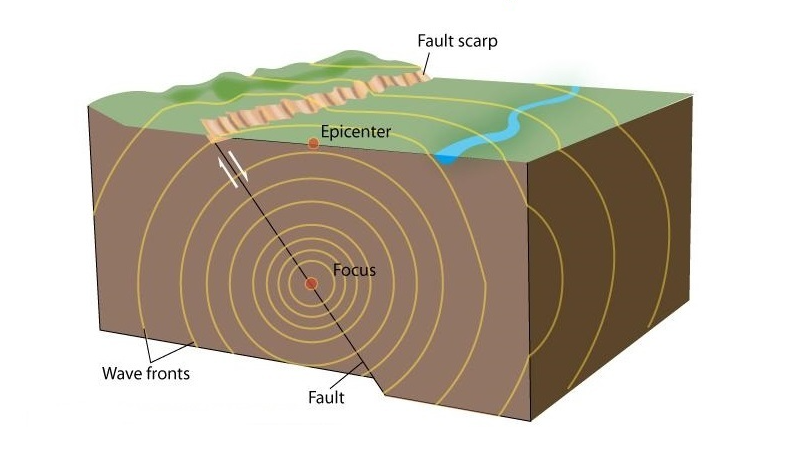
\includegraphics[height=4cm]{Diapos/Intro/Figures/natural_seismicity}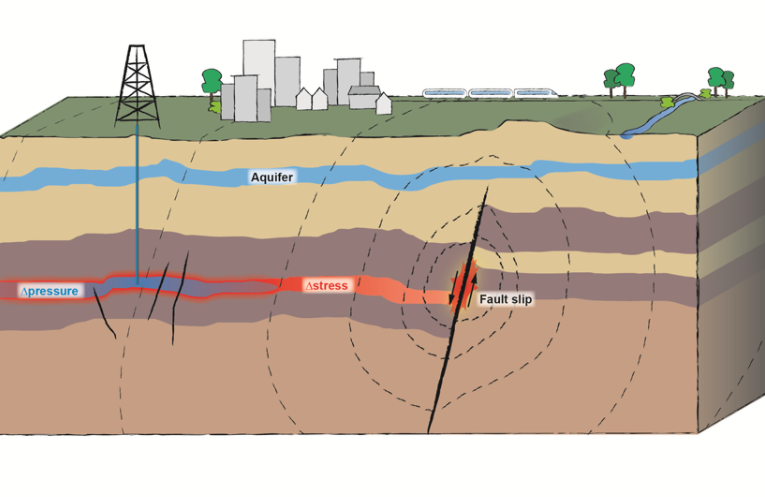
\includegraphics[height=4cm]{Diapos/Intro/Figures/induced_seismicity}\\

\vspace{-0.35cm}
\center\scriptsize{Natural seismicity  \textit{(Source: sciencelearn.org.nz)} and induced seismicity \textit{(Source: eos.org)}.}

\vspace{1cm}
\raggedright\normalsize{Knowing the hazard of each area is essential to estimate and prevent the effect of earthquakes.}
%\includegraphics[height=0.11\textheight]{./logos/logo_upv.jpg} \hspace*{0.2cm}
%includegraphics[height=0.11\textheight]{./logos/logo_bcam.jpg} \hspace*{0.2cm}
\end{frame} 

%%%%%%%%%%%%%%%%%%%%%%%%%%%%%%%%

\begin{frame}{Geophysical Applications: Energy  $\&$ Climate Change}

%\titlepage
\vspace{-0.2cm}
\center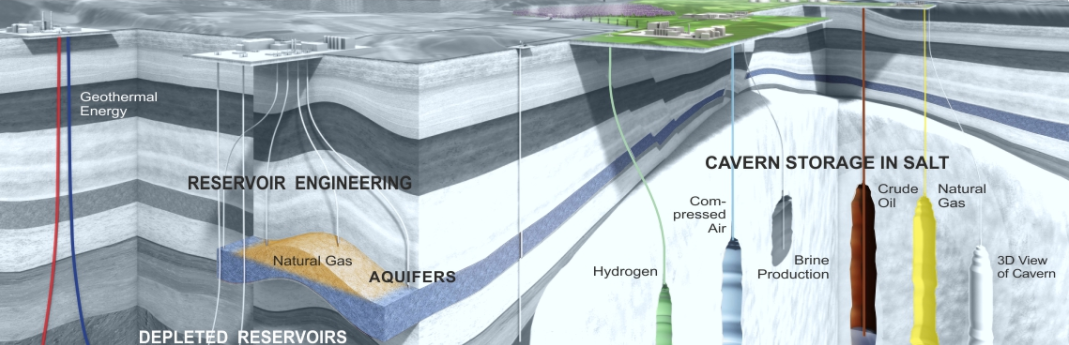
\includegraphics[height=4cm]{Diapos/Intro/Figures/Room_for_energy} \hspace*{0.2cm}\\
\vspace{-0.35cm}
\center\scriptsize{Source: https://deep-kbb.de/}

\vspace{1cm}
\raggedright\normalsize{\textbf{Geothermal energy, oil and gas exploitation, H$_2$  $\&$ CO$_2$ storage} require characterization and monitoring of the Earth's subsurface.}
%\includegraphics[height=0.11\textheight]{./logos/logo_upv.jpg} \hspace*{0.2cm}
%includegraphics[height=0.11\textheight]{./logos/logo_bcam.jpg} \hspace*{0.2cm}
\end{frame} 

%%%%%%%%%%%%%%%%%%%%%%%%%%%%%%%%

\begin{frame}{Exploration Method: Geosteering}

%\titlepage
\vspace{0.1cm}
\center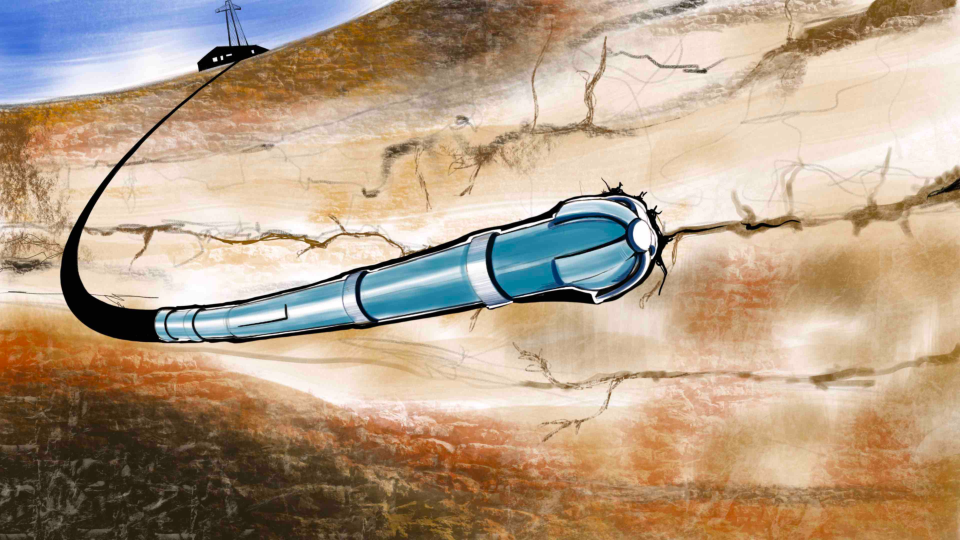
\includegraphics[height=3cm, width=10cm]{Diapos/Intro/Figures/Geosteering_drawing} \hspace*{0.2cm}\\
%\vspace{-0.35cm}
%\center\scriptsize{Source: https://deep-kbb.de/}

\vspace{0.4cm}
\raggedright\normalsize{\textbf{Geosteering.} The act of adjusting the borehole position in \textbf{real-time} to reach one or more targets.}

\visible<2>{
\begin{figure}
\centering
	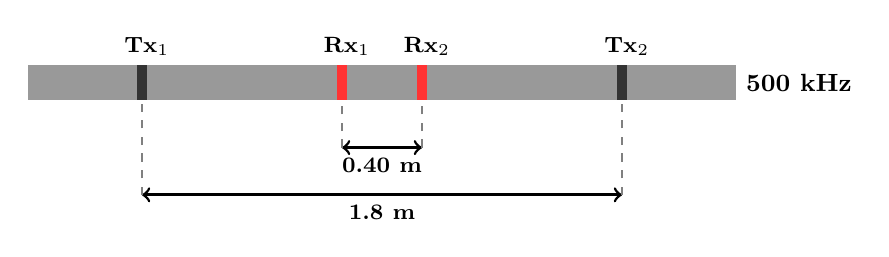
\begin{tikzpicture}

%% Tool
\fill[gray!80!white] (-1.5*3,0) -- (1.5*3,0.) --  node[right] {\small \bf \textcolor{black}{500 kHz}}  (1.5*3, 0.15*3) -- (-1.5*3,0.15*3) -- cycle;

%% Transmitters
\fill[black!80!white] (-0.6096*5-0.02*3,0) -- (-0.6096*5+0.02*3,0.) -- (-0.6096*5+0.02*3, 0.15*3) node[above] {\footnotesize \bf \textcolor{black}{Tx$_1$}}  -- (-0.6096*5-0.02*3,0.15*3) -- cycle;
%
\fill[black!80!white] (0.6096*5-0.02*3,0) -- (0.6096*5+0.02*3,0.)  -- (0.6096*5+0.02*3, 0.15*3) node[above] {\footnotesize \bf \textcolor{black}{Tx$_2$}} -- (0.6096*5-0.02*3,0.15*3) -- cycle;

%% Receivers
\fill[red!80!white] (-0.1016*5-0.02*3,0) -- (-0.1016*5+0.02*3,0.)  -- (-0.1016*5+0.02*3, 0.15*3) node[above] {\footnotesize \bf \textcolor{black}{Rx$_1$}} -- (-0.1016*5-0.02*3,0.15*3) -- cycle;
\fill[red!80!white] ( 0.1016*5-0.02*3,0) -- ( 0.1016*5+0.02*3,0.) -- ( 0.1016*5+0.02*3, 0.15*3)  node[above] {\footnotesize \bf \textcolor{black}{Rx$_2$}} -- ( 0.1016*5-0.02*3,0.15*3) -- cycle;

%% distances
\draw[black, line width=1pt,<->] (-0.1016*5, -0.6)      -- (0.1016*5, -0.6) node[pos=0.5, below] {\footnotesize \bf \textcolor{black}{0.40 m}}  ;
\draw[gray, dashed] (-0.1016*5, -0.6)      -- (-0.1016*5, 0)  ;
\draw[gray, dashed] ( 0.1016*5, -0.6)      -- ( 0.1016*5, 0)  ;

\draw[black, line width=1pt,<->] (-0.6096*5, -1.2)      -- (0.6096*5, -1.2) node[pos=0.5, below] {\footnotesize \bf \textcolor{black}{1.8 m}}  ;
\draw[gray, dashed] (-0.6096*5,-1.2)      -- (-0.6096*5, 0)  ;
\draw[gray, dashed] ( 0.6096*5,-1.2)      -- ( 0.6096*5, 0)  ;


\end{tikzpicture}
\end{figure}
}
\end{frame} 
